\section{Topics covered}
\begin{itemize}
  \item Software process models
  \item Process activities
  \item Coping with change
  \item The Rational Unified Process(\textit{An example of a modern software process}).

\end{itemize}

\section{The software process}
\begin{itemize}
  \item A structured set of activities required to develop a software system.
  \item Many different software processes but all involve:
  \begin{enumerate}
    \item Specification $-$ defining what the system should do;
    \item Design and implementation $-$ defining the organization of the system and implementing the system;
    \item Validation $-$ checking that it does what the customer wants;
    \item Evolution $-$ changing the system in response to changing customer needs.
  \end{enumerate}

  \item A software process model is an abstract representation of a process. It presents a description of a process from some particular perspective.
\end{itemize}


\subsection{Software process descriptions}

\begin{itemize}
  \item When we describe and discuss processes, we usually talk about the activities in these processes such as specifying a data model, designing a user interface, etc. and the ordering of these activities.
  \item Process descriptions may also include:
  \begin{enumerate}
    \item Products, which are the outcomes of a process activity;
    \item Roles, which reflect the responsibilities of the people involved in the process;
    \item Pre- and post-conditions, which are statements that are true before and after a process activity has been enacted or a product produced.
  \end{enumerate}

\end{itemize}

\section{Plan-driven and agile processes}

  \begin{itemize}
    \item Plan-driven processes are processes where all of the process activities are planned in advance and progress is measured against this plan.
    \item In agile processes, planning is incremental and it is easier to change the process to reflect changing customer requirements.
    \item In practice, most practical processes include elements of both plan-driven and agile approaches.
    \item There are no right or wrong software processes.
  \end{itemize}

\section{Software process models}
\begin{enumerate}
  \item \textbf{The waterfall model} Plan-driven model. Separate and distinct phases of specification and development.

  \item \textbf{Incremental development} Specification, development and validation are interleaved. May be plan-driven or agile.

  \item \textbf{Reuse-oriented software engineering} The system is assembled from existing components. May be plan-driven or agile.

  \item In practice, most large systems are developed using a process that incorporates elements from all of these models.
\end{enumerate}
\newpage
\subsection{The Waterfall Model}
\begin{figure}[h!]
    \centering
    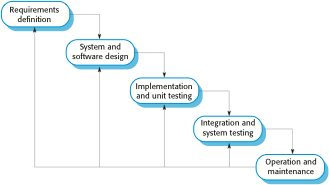
\includegraphics[width = 0.8\textwidth]{./figures/waterfall_L1_1.png}
    \caption{}
    \label{fig:L1_1}
\end{figure}

\subsubsection{Waterfall model phases}
\begin{itemize}
  \item There are separate identified phases in the waterfall model:
  \begin{enumerate}
    \item Requirements analysis and definition
    \item System and software design
    \item Implementation and unit testing
    \item Integration and system testing
    \item Operation and maintenance
  \end{enumerate}
  \item The main drawback of the waterfall model is the difficulty of accommodating change after the process is underway. In principle, a phase has to be complete before moving onto the next phase.

\end{itemize}


\subsubsection{Waterfall model problems}
\begin{itemize}
  \item Inflexible partitioning of the project into distinct stages makes it difficult to respond to changing customer requirements.
  \begin{itemize}
    \item Therefore, this model is only appropriate when the requirements are well-understood and changes will be fairly limited during the design process.
    \item Few business systems have stable requirements.
  \end{itemize}

  \item The waterfall model is mostly used for large systems engineering projects where a system is developed at several sites.
  \newline
  In those circumstances, the plan-driven nature of the waterfall model helps coordinate the work.
  Incremental development

\end{itemize}
\subsection{Incremental development}
\begin{figure}[h!]
    \centering
    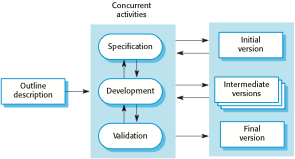
\includegraphics[width = 0.8\textwidth]{./figures/Incrementaldevelopment_L1_2.png}
    \caption{}
    \label{fig:L1_2}
\end{figure}

\subsubsection{Incremental development benefits}
\begin{itemize}
  \item The cost of accommodating changing customer requirements is reduced.
  \newline The amount of analysis and documentation that has to be redone is much less than is required with the waterfall model.
  \item It is easier to get customer feedback on the development work that has been done.
  \newline Customers can comment on demonstrations of the software and see how much has been implemented.
  \item More rapid delivery and deployment of useful software to the customer is possible.
  \newline Customers are able to use and gain value from the software earlier than is possible with a waterfall process.
\end{itemize}

\subsubsection{Incremental development problems}
\begin{itemize}
  \item The process is not visible.
  \newline Managers need regular deliverables to measure progress. If systems are developed quickly, it is not cost-effective to produce documents that reflect every version of the system.

  \item System structure tends to degrade as new increments are added.
  \newline Unless time and money is spent on refactoring to improve the software, regular change tends to corrupt its structure. Incorporating further software changes becomes increasingly difficult and costly.
\end{itemize}

\subsection{Reuse-oriented software engineering}
\begin{itemize}
  \item Based on systematic reuse where systems are integrated from existing components or COTS (Commercial-off-the-shelf) systems.
  \item Process stages
  \begin{enumerate}
    \item Component analysis
    \item Requirements modification
    \item System design with reuse
    \item Development and integration.
  \end{enumerate}
  \item Reuse is now the standard approach for building many types of business system
  \newline Reuse covered in more depth in Chapter 16.
\end{itemize}



\subsubsection{Reuse-oriented software engineering}
\begin{figure}[h!]
    \centering
    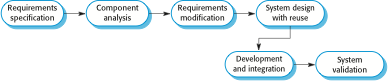
\includegraphics[width = 0.8\textwidth]{./figures/Reuse-oriented_L1_3.png}
    \caption{}
    \label{fig:L1_3}
\end{figure}



\section{Types of software component}
\begin{itemize}

\item Web services that are developed according to service standards and which are available for remote invocation.

\item Collections of objects that are developed as a package to be integrated with a component framework such as .NET or J2EE.

\item Stand-alone software systems (COTS) that are configured for use in a particular environment.
\end{itemize}

\section{Process activities}
\begin{itemize}
\item Real software processes are inter-leaved sequences of technical, collaborative and managerial activities with the overall goal of specifying, designing, implementing and testing a software system.

\item The four basic process activities of specification, development, validation and evolution are organized differently in different development processes. In the waterfall model, they are organized in sequence, whereas in incremental development they are inter-leaved.
\end{itemize}

\section{Software specification}
\begin{itemize}

\item The process of establishing what services are required and the constraints on the system’s operation and development.

\item Requirements engineering process
\begin{enumerate}

\item Feasibility study
\newline
-Is it technically and financially feasible to build the system? \newline
\item Requirements elicitation and analysis
-What do the system stakeholders require or expect from the system? \newline
\item Requirements specification
-Defining the requirements in detail \newline
\item Requirements validation
-Checking the validity of the requirements
\end{enumerate}

\end{itemize}

\newpage
\section{The requirements engineering process}
\begin{figure}[h!]
    \centering
    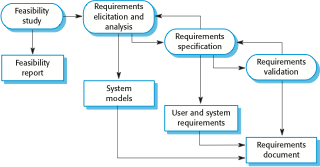
\includegraphics[width = 0.8\textwidth]{./figures/requirements_L1_4.png}
    \caption{}
    \label{fig:L1_4}
\end{figure}



\section{Software design and implementation}
\begin{itemize}

\item The process of converting the system specification into an executable system.

\item Software design
\newline $-$Design a software structure that realises the specification;
\item Implementation
\newline $-$Translate this structure into an executable program;

\item The activities of design and implementation are closely related and may be inter-leaved.
\end{itemize}

\newpage
\section{A general model of the design process}
\begin{figure}[h!]
    \centering
    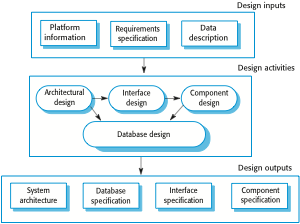
\includegraphics[width = 0.8\textwidth]{./figures/designprocess_L1_5.png}
    \caption{}
    \label{fig:L1_5}
\end{figure}


\section{Design activities}
\begin{itemize}

\item Architectural design, where you identify the overall structure of the system, the principal components (sometimes called sub-systems or modules), their relationships and how they are distributed.

\item Interface design, where you define the interfaces between system components.

\item Component design, where you take each system component and design how it will operate.

\item Database design, where you design the system data structures and how these are to be represented in a database.
\end{itemize}

\section{Software validation}
\begin{itemize}
\item Verification and validation (V \& V) is intended to show that a system conforms to its specification and meets the requirements of the system customer.
\item Involves checking and review processes and system testing.
\item System testing involves executing the system with test cases that are derived from the specification of the real data to be processed by the system.
\item Testing is the most commonly used V \& V activity.
\end{itemize}



\section{Stages of testing}
\begin{figure}[h!]
    \centering
    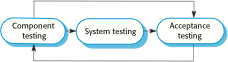
\includegraphics[width = 0.8\textwidth]{./figures/stagesoftesting_L1_6.png}
    \caption{}
    \label{fig:L1_6}
\end{figure}


\subsection{Testing stages}
\begin{itemize}
\item Development or component testing \item Individual components are tested independently;
\item Components may be functions or objects or coherent groupings of these entities.

\item System testing

\item Testing of the system as a whole. Testing of emergent properties is particularly important.

\item Acceptance testing

\item Testing with customer data to check that the system meets the customer’s needs.
\end{itemize}

\newpage
\subsection{Testing phases in a plan-driven software process}
\begin{figure}[h!]
    \centering
    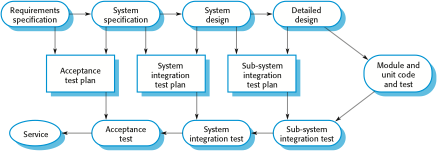
\includegraphics[width = 0.8\textwidth]{./figures/testing_phases_L1_7.png}
    \caption{}
    \label{fig:L1_7}
\end{figure}




\section{Software evolution}
\begin{itemize}

\item Software is inherently flexible and can change.

\item As requirements change through changing business circumstances, the software that supports the business must also evolve and change.

\item Although there has been a demarcation between development and evolution (maintenance) this is increasingly irrelevant as fewer and fewer systems are completely new.
\end{itemize}

\newpage
\section{System evolution}
\begin{figure}[h!]
    \centering
    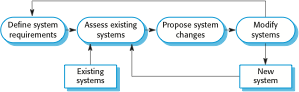
\includegraphics[width = 0.8\textwidth]{./figures/systemevolution_L1_8.png}
    \caption{}
    \label{fig:L1_8}
\end{figure}

\section{Key points}
\begin{itemize}

\item Software processes are the activities involved in producing a software system. Software process models are abstract representations of these processes.

\item General process models describe the organization of software processes. Examples of these general models include the ‘waterfall’ model, incremental development, and reuse-oriented development.

\item Requirements engineering is the process of developing a software specification.

\item Design and implementation processes are concerned with transforming a requirements specification into an executable software system.

\item Software validation is the process of checking that the system conforms to its specification and that it meets the real needs of the users of the system.

\item Software evolution takes place when you change existing software systems to meet new requirements. The software must evolve to remain useful.
\end{itemize}

\section{Coping with change}
\begin{itemize}
\item Change is inevitable in all large software projects.

\item Business changes lead to new and changed system requirements
\item New technologies open up new possibilities for improving implementations
\item Changing platforms require application changes

\item Change leads to rework so the costs of change include both rework (e.g. re-analysing requirements) as well as the costs of implementing new functionality
\end{itemize}

\section{Reducing the costs of rework}
\begin{itemize}
\item Change avoidance, where the software process includes activities that can anticipate possible changes before significant rework is required.

\item For example, a prototype system may be developed to show some key features of the system to customers.

\item Change tolerance, where the process is designed so that changes can be accommodated at relatively low cost.

\item This normally involves some form of incremental development. Proposed changes may be implemented in increments that have not yet been developed. If this is impossible, then only a single increment (a small part of the system) may have be altered to incorporate the change.
\end{itemize}


\section{Software prototyping}
\begin{itemize}
\item A prototype is an initial version of a system used to demonstrate concepts and try out design options.

\item A prototype can be used in:

\item The requirements engineering process to help with requirements elicitation and validation;
\item In design processes to explore options and develop a UI design; \item In the testing process to run back-to-back tests.
\end{itemize}


\subsection{Benefits of prototyping}
\begin{itemize}
\item Improved system usability.

\item A closer match to users' real needs.

\item Improved design quality.

\item Improved maintainability.

\item Reduced development effort.
\end{itemize}

\subsection{The process of prototype development}
\begin{figure}[h!]
    \centering
    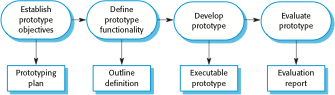
\includegraphics[width = 0.8\textwidth]{./figures/prototype_L1_9.png}
    \caption{}
    \label{fig:L1_9}
\end{figure}


\subsection{Prototype development}
\begin{itemize}
\item May be based on rapid prototyping languages or tools
\item May involve leaving out functionality
\item Prototype should focus on areas of the product that are not well-understood;
\item Error checking and recovery may not be included in the prototype;
\item Focus on functional rather than non-functional requirements such as reliability and security
\end{itemize}

\subsection{Throw-away prototypes}
\begin{itemize}
\item Prototypes should be discarded after development as they are not a good basis for a production system:

\item It may be impossible to tune the system to meet non-functional requirements;
\item Prototypes are normally undocumented;

\item The prototype structure is usually degraded through rapid change;
\item The prototype probably will not meet normal organisational quality standards.
\end{itemize}


\section{Incremental delivery}
\begin{itemize}
\item Rather than deliver the system as a single delivery, the development and delivery is broken down into increments with each increment delivering part of the required functionality.

\item User requirements are prioritised and the highest priority requirements are included in early increments.

\item Once the development of an increment is started, the requirements are frozen though requirements for later increments can continue to evolve.
\end{itemize}

\section{Incremental development and delivery}
\begin{itemize}
\item Incremental development
\item Develop the system in increments and evaluate each increment before proceeding to the development of the next increment;
\item Normal approach used in agile methods; \item Evaluation done by user/customer proxy.
\item Incremental delivery

\item Deploy an increment for use by end-users;

\item More realistic evaluation about practical use of software;

\item Difficult to implement for replacement systems as increments have less functionality than the system being replaced.
\end{itemize}
% \newpage
\section{Incremental delivery}
\begin{figure}[h!]
    \centering
    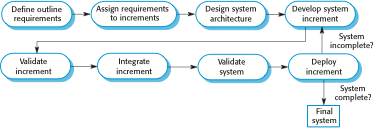
\includegraphics[width = 0.8\textwidth]{./figures/L1_10.png}
    \caption{}
    \label{fig:L1_10}
\end{figure}


\section{Incremental delivery advantages}
\begin{itemize}
\item Customer value can be delivered with each increment so system functionality is available earlier.

\item Early increments act as a prototype to help elicit requirements for later increments.

\item Lower risk of overall project failure.

\item The highest priority system services tend to receive the most testing.
\end{itemize}

\section{Incremental delivery problems}
\begin{itemize}

\item Most systems require a set of basic facilities that are used by different parts of the system.
\item As requirements are not defined in detail until an increment is to be implemented, it can be hard to identify common facilities that are needed by all increments.
\item The essence of iterative processes is that the specification is developed in conjunction with the software.
\item However, this conflicts with the procurement model of many organizations, where the complete system specification is part of the system development contract.
\end{itemize}

\section{Boehm’s spiral model}

\begin{itemize}
\item Process is represented as a spiral rather than as a sequence of activities with backtracking.
\item Each loop in the spiral represents a phase in the process.
\item No fixed phases such as specification or design - loops in the spiral are chosen depending on what is required.
\item Risks are explicitly assessed and resolved throughout the process.
\end{itemize}

\section{Boehm’s spiral model of the software process}
\begin{figure}[h!]
    \centering
    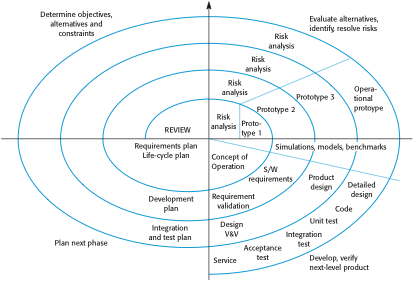
\includegraphics[width = 0.8\textwidth]{./figures/L1_11.png}
    \caption{}
    \label{fig:L1_11}
\end{figure}



\section{Spiral model sectors}
\begin{itemize}
\item Objective setting

\item Specific objectives for the phase are identified. \item Risk assessment and reduction
\item Risks are assessed and activities put in place to reduce the key risks.

\item Development and validation

\item A development model for the system is chosen which can be any of the generic models.

\item Planning

\item The project is reviewed and the next phase of the spiral is planned.
\end{itemize}

\section{Spiral model usage}
\begin{itemize}

\item Spiral model has been very influential in helping people think about iteration in software processes and introducing the risk-driven approach to development.

\item In practice, however, the model is rarely used as published for practical software development.
\end{itemize}

\section{The Rational Unified Process}
\begin{itemize}
\item A modern generic process derived from the work on the UML and associated process.

\item Brings together aspects of the 3 generic process models discussed previously.

\item Normally described from 3 perspectives

\item A dynamic perspective that shows phases over time; \item A static perspective that shows process activities; \item A practive perspective that suggests good practice.
\end{itemize}

\newpage
\section{Phases in the Rational Unified Process}
\begin{figure}[h!]
    \centering
    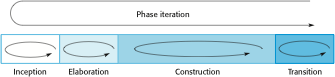
\includegraphics[width = 0.8\textwidth]{./figures/L1_12.png}
    \caption{}
    \label{fig:L1_12}
\end{figure}


\section{RUP phases}
\begin{itemize}
\item Inception

\item Establish the business case for the system. \item Elaboration
\item Develop an understanding of the problem domain and the system architecture.

\item Construction

\item System design, programming and testing.
\item Transition
\item Deploy the system in its operating environment.
\end{itemize}

\section{RUP iteration}
\begin{itemize}
\item In-phase iteration

\item Each phase is iterative with results developed incrementally. \item Cross-phase iteration
\item As shown by the loop in the RUP model, the whole set of phases may be enacted incrementally.
\end{itemize}
\newpage
\section{Static workflows in the Rational Unified Process}
\begin{table}[h!]
\centering
\begin{tabular}{ |p{3cm}|p{7cm}|  }
\hline
Workflow & Description  \\
\hline
Business modelling
& The business processes are modelled using business use cases.\\
\hline
Requirements
& Actors who interact with the system are identified and use cases are developed to model the system requirements.\\
\hline
Analysis and design
& A design model is created and documented using architectural models, component models, object models and sequence models.\\
\hline
Implementation
& The components in the system are implemented and structured	into	implementation	sub-systems. Automatic code generation from design models helps accelerate this process.\\
\hline
\end{tabular}

\label{table:T1_1}
\end{table}

\newpage
\section{Static workflows in the Rational Unified Process}
\begin{table}[h!]
\centering
\begin{tabular}{ |p{3cm}|p{7cm}|  }
\hline
Workflow & Description  \\
\hline
Testing & Testing is an iterative process that is carried out in conjunction with implementation. System testing follows the completion of the implementation.\\
\hline
Deployment & A product release is created, distributed to users and installed in their workplace. \\
\hline
Configuration	and change management & This supporting workflow managed changes to the system (see Chapter 25). \\
\hline
Project management & This supporting workflow manages the system development (see Chapters 22 and 23). \\
\hline
Environment & This workflow is concerned with making appropriate software tools available to the software development team. \\
\hline
\end{tabular}

\label{table:T1_2}
\end{table}

\section{RUP good practice}
\begin{itemize}

\item Develop software iteratively

\item Plan increments based on customer priorities and deliver highest priority increments first.

\item Manage requirements
% \item Explicitly document customer requirements and keep track of changes to these requirements.
\item Use component-based architectures

\item Organize the system architecture as a set of reusable components.
\end{itemize}

\section{RUP good practice}
\begin{itemize}

\item Visually model software

\item Use graphical UML models to present static and dynamic views of the software.

\item Verify software quality

\item Ensure that the software meet’s organizational quality standards. \item Control changes to software
\item Manage software changes using a change management system and configuration management tools.
\end{itemize}

\section{Key points}
\begin{itemize}
\item Processes should include activities to cope with change. This may involve a prototyping phase that helps avoid poor decisions on requirements and design.

\item Processes may be structured for iterative development and delivery so that changes may be made without disrupting the system as a whole.

\item The Rational Unified Process is a modern generic process model that is organized into phases (inception, elaboration, construction and transition) but separates activities (requirements, analysis and design, etc.) from these phases.
\end{itemize}
